\subsubsection{Logic contracts}
In this section are illustrated the logic contracts of \textit{Soldino}, these contracts implement a substantial part of the business logic, in fact they define inputs validation mechanics, events to be emitted on the blockchain when a state change is made and comunicate with each other.
For the comunication part, since logic contracts are upgradeable, every logic contract has a \texttt{ContractManager} state variable, used to get the latest address of another contract. In this way the coupling between logic contract is minimum and there's no need to maintain correct references in each logic contract.\\
However each \texttt{xLogic} contract has a direct reference to its \texttt{xStorage} contract because the latter is immutable.
\pagebreak
\paragraph{UserLogic}\mbox{}\\

\noindent This contract provides an interface to comunicate with the \texttt{UserStorage} contract. \texttt{addCitizen} and \texttt{addBusiness} functions add a new user and set its type depending on which function is called.
\begin{figure}[H]
	\centering
	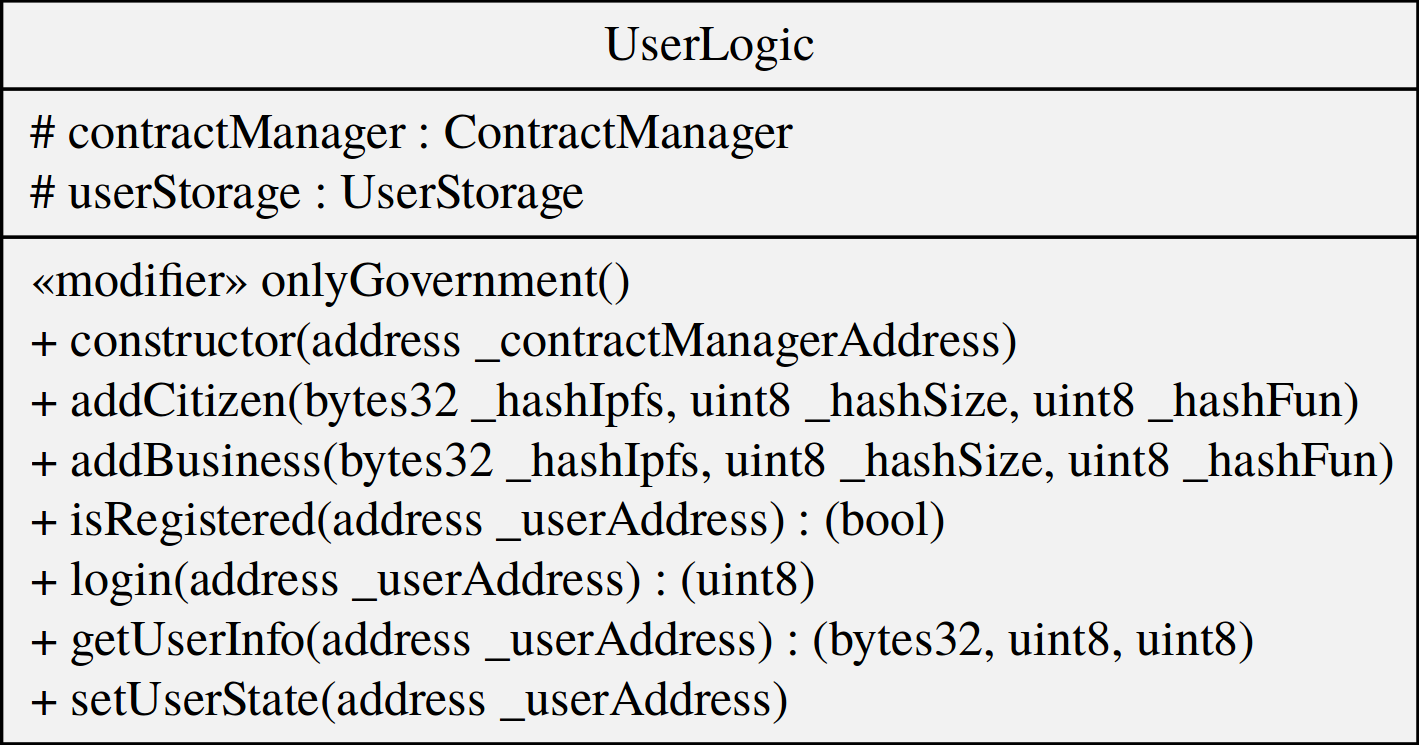
\includegraphics[scale=0.20]{res/images/solidity/userlogic.png}
	\caption{class diagram of the UserLogic contract}
\end{figure}

\paragraph{ProductLogic}\mbox{}\\

\noindent This contract allow business to insert new products, modify or delete exiting ones. Obviously only businesses can insert products in \textit{Soldino}, to check this invariant \texttt{ProductLogic} defines the modifier \texttt{onlyBusiness} which check if the address trying to insert a product is a business. Furthermore, products can be modified and deleted only by their sellers and the modifier \texttt{onlyProductOwner} checks that.
\begin{figure}[H]
	\centering
	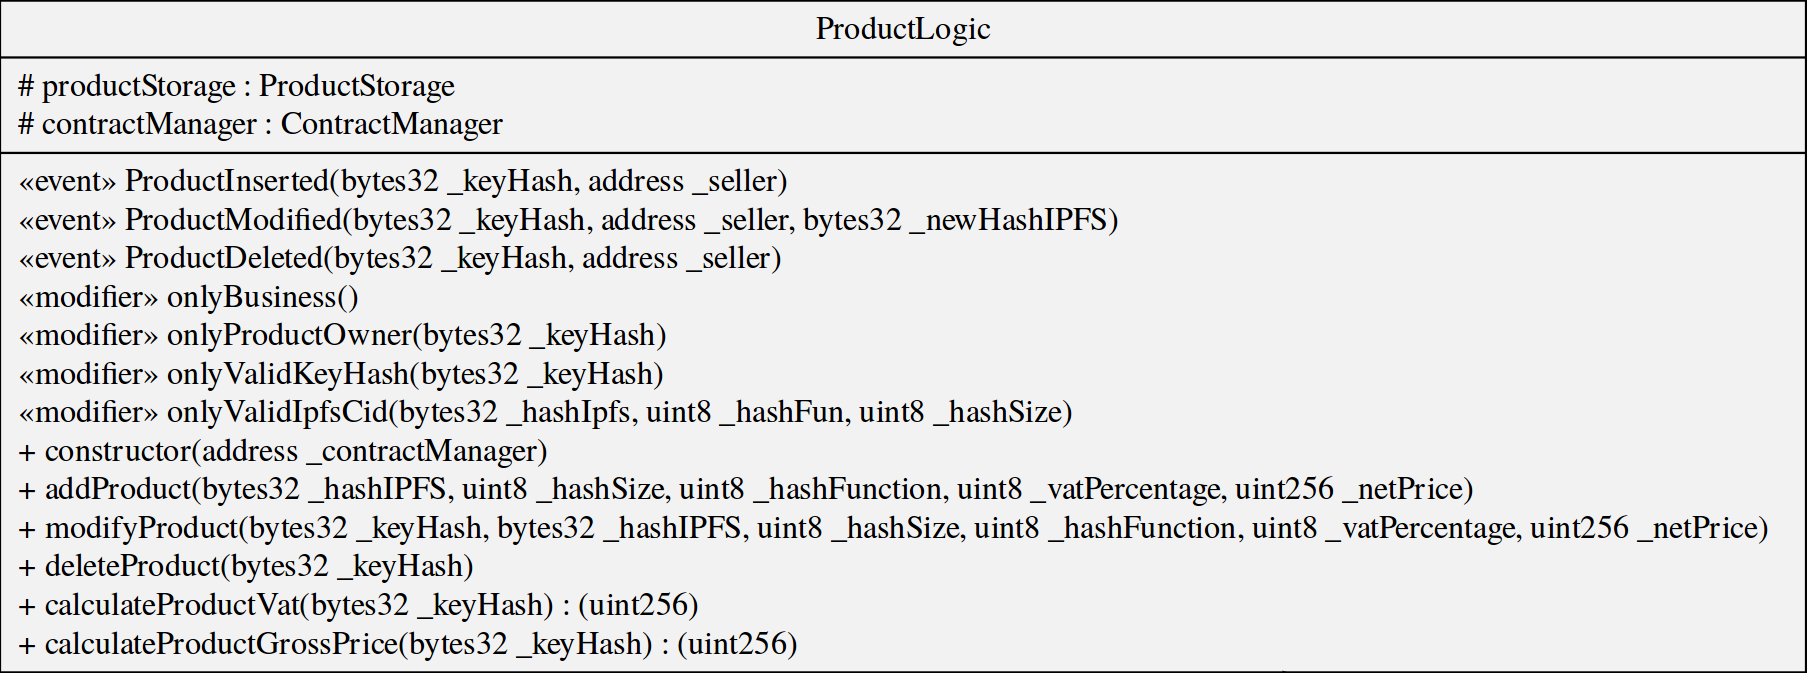
\includegraphics[scale=0.25]{res/images/solidity/productlogic.png}
	\caption{class diagram of the ProductLogic contract}
\end{figure}

\paragraph{VatLogic}\mbox{}\\

\no
\begin{figure}[H]
	\centering
	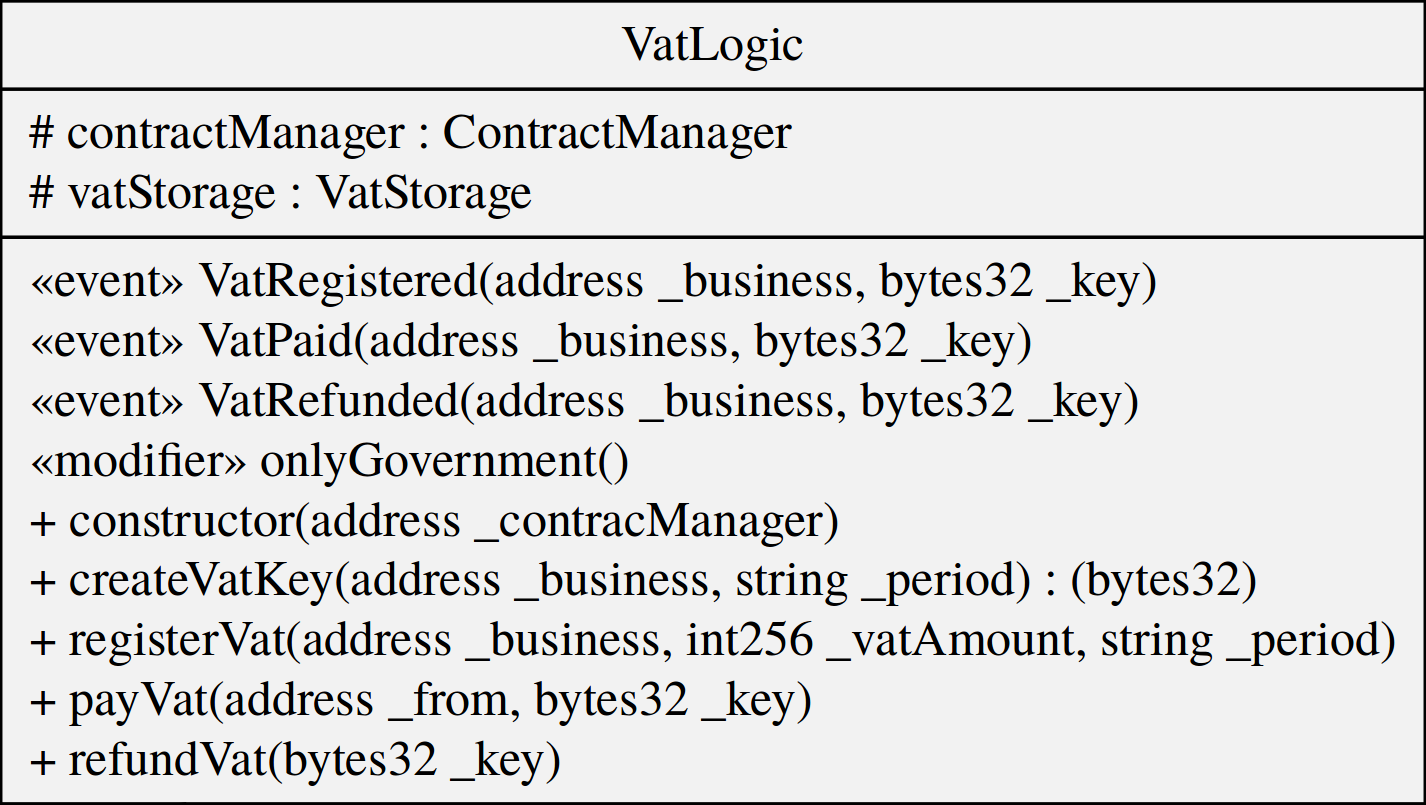
\includegraphics[scale=0.20]{res/images/solidity/vatlogic.png}
	\caption{class diagram of the VatLogic contract}
\end{figure}

\paragraph{OrderLogic}\mbox{}\\
\begin{figure}[H]
	\centering
	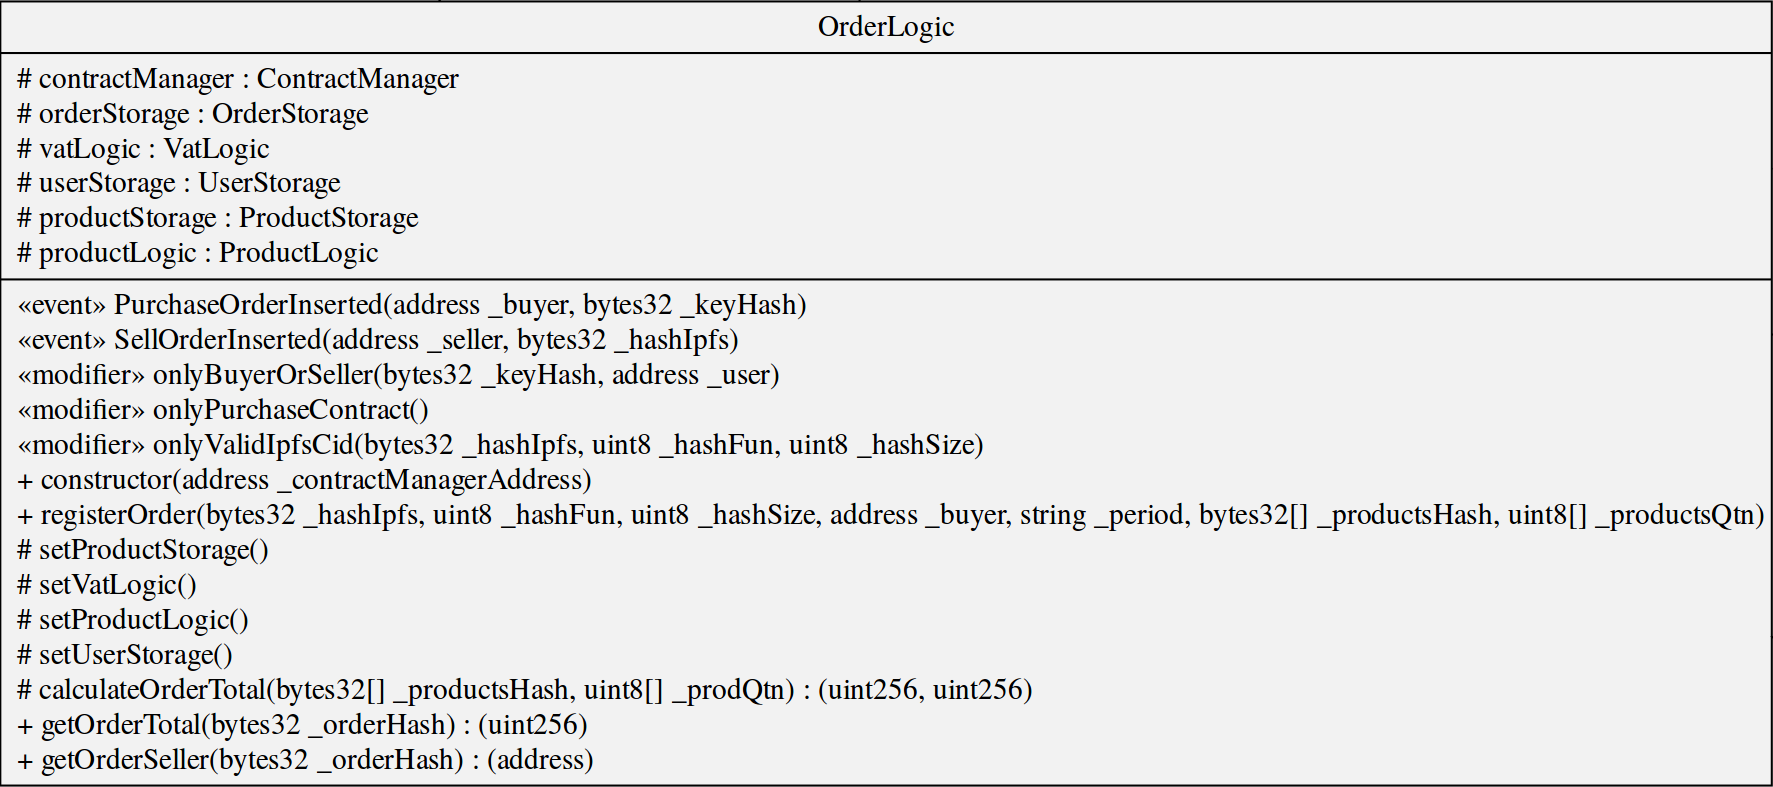
\includegraphics[scale=0.25]{res/images/solidity/orderlogic.png}
	\caption{class diagram of the OrderLogic contract}
\end{figure}